\chapter{Implementatie}
\section{Inleiding}
Na de literatuurstudie en de ontwerpfase, moet het ontwerp dat besproken werd in het vorige hoofdstuk geïmplementeerd worden.
Als programmeertaal werd Python gekozen.
In het bedrijf is een zeker kennis van Python aanwezig waardoor de overname vlotter zal verlopen.
Het doel is om een programma te ontwikkelen dat de belangrijkste functies omvat en dat gemakkelijk uitgebreid kan worden.
In de komende secties worden de verschillende implementatie beslissingen toegelicht en wordt de geschreven code toegelicht.
In wat volgt, zullen de server-side en client-side van elkaar gescheiden worden en afzonderlijk besproken worden.
De verschillende Python modules worden overlopen en alle methodes met speciale kenmerken worden toegelicht.

\section{Installeren van de software}

\section{Server-side}
\subsection{deployment\_server}
Zoals werd aangegeven in Hoofdstuk~\ref{sec:initServer} bestaat het opstarten van een server uit het creëren van een ReleaseDock object gevolgd door het creëren van een Broker object.
Vervolgens gaat het release dock zich inschrijven voor de nodige berichten (zie Figuur~\vref{fig:seqStartServerNew}).

\begin{figure}[!ht]
\centering
\makebox[0pt]{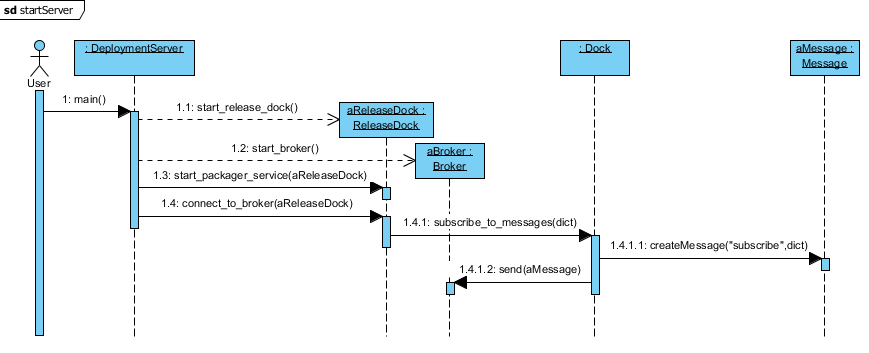
\includegraphics[width=\textwidth]{afbeelding/seqStartServer.png}}
\caption{Sequentie diagram voor het opstarten van een server}
\label{fig:seqStartServerNew}
\end{figure}

Bij het opstarten van de docks moeten verschillende parameters meegegeven worden.
Listing~\ref{list:startServer} geeft weer welke parameters ingevuld moeten worden voor een correcte functionaliteit.
De broker interface en port worden gebruikt door de Broker om een socket te openen maar ook door ReleaseDock om te connecteren met de broker.
De release\_dock interface en port zijn bedoelt voor in de ReleaseDock een socket te openen waar de Broker berichten naar kan verzenden.
Als laatste moeten de release interface en port gespecificeerd worden.
Met deze variabelen wordt een socket geopend die gebruikt wordt door het FieldDock om een installer op te halen\footnote{Het ophalen van een installer is het enige moment waarop een FieldDock direct connecteert met een ReleaseDock}.			

\begin{minipage}{\linewidth}
\begin{center}
%\lstset{language=Python}
\begin{lstlisting}[caption={Parameters voor server en broker},label={list:startServer}]
    broker_interface = "10.129.58.139"
    broker_port = 12347
    release_dock_interface = "10.129.58.139"
    release_dock_port = 12345
    release_interface = "10.129.58.139"
    release_port = 12346
\end{lstlisting}
\end{center}
\end{minipage}

\subsection{dock}
\paragraph{Starten van de services} %-> queue systeem uitleggen
Na het creëren van een dock moeten verscheidene acties uitgevoerd worden.
Zo zal een ReleaseDock een connectie met een databank opstarten en een FieldDock zal een connectie maken met de Docker client.
Uit het klassendiagram in Figuur~\vref{fig:classDiagram} bleek al dat beide klassen methodes overerven van de Dock klasse.
Ieder Dock object moet dan ook in staat zijn om binnenkomende berichten correct af te kunnen handelen.
Om deze taak uit te voeren, worden twee threads opgestart (zie Listing~\vref{list:startService}).

\begin{minipage}{\linewidth}
\begin{center}
%\lstset{language=Python}(*@\centerline{\raisebox{-1pt}[0pt][0pt]{$\vdots$}}@*)
\begin{lstlisting}[caption={Starten van dock services},label={list:startService}]
    self.open_socket()
    thread = Thread(target=self.listen_for_data, args=())
    thread.daemon = True
    thread.start()

    message_thread = Thread(target=self.handle_message, args=())
    message_thread.daemon = True
    message_thread.start()
\end{lstlisting}
\end{center}
\end{minipage}

De listen\_for\_data methode wacht continue op het toekomen van data op de socket.
Van zodra data toekomt, wordt deze in een Queue object gestoken.
Zowel het accepteren van een inkomende connectie als het verwijderen van een object uit de queue zijn blocking methodes.
Dit wil zeggen dat zolang er geen binnenkomende connecties zijn en zolang er geen objecten in de queue zitten, zullen deze threads ook niks doen.
De threads worden geblockt totdat de juiste acties uitgevoerd worden.

\begin{minipage}{\linewidth}
\begin{center}
\lstset{escapeinside={(*@}{@*)}}
\begin{lstlisting}[caption={Ontvangen en afhandelen van data},label={list:receiveData}]
    def listen_for_data(self):
        while True:
            conn, address = self.message_socket.accept()
            print("DOCK -- Connected by \n\t\t" + str(address))
(*@\centerline{\raisebox{-1pt}[0pt][0pt]{$\vdots$}}@*)
            data = conn.recv(1024)
            print("DOCK -- received data: \n\t\t" + data)
            self.message_queue.put(data)
            
    def handle_message(self):
        while True:
            data = self.message_queue.get()
(*@\centerline{\raisebox{-1pt}[0pt][0pt]{$\vdots$}}@*)
\end{lstlisting}
\end{center}
\end{minipage}

\subsection{release\_dock}
\paragraph{Kopiëren van bestanden} %-> Copy old meta folder
Tijdens het creëren van een installer wordt gecontroleerd of een geselecteerd pakket al bestaat.
Mocht dit het geval zijn dan moeten de nodige bestanden uit de originele meta-data folder gekopieerd worden naar de nieuwe locatie.
Om dit uit te voeren, wordt er gebruik gemaakt van de copy\_tree methode uit de distutils module.
De doellocatie wordt door deze methode overschreven met bestanden uit de oorspronkelijke locatie.

\paragraph{Agenten verzenden}
Een onderdeel van het deploymentproces bestaat uit het kopiëren van de nodige agenten naar het field dock.
Om dit uit te voeren wordt Dill\footnote{\url{https://pypi.python.org/pypi/dill}} gebruikt om de nodige objecten te serialiseren en deserialiseren.
Listing~\vref{list:serDeser} geeft de code weer die hiervoor gebruikt wordt.
De dill.dumps methode zorgt ervoor dat het object omgezet wordt naar een string die kan worden verzonden over een socket.
Om dit correct uit te voeren wordt eerst de lengte van de string verzonden zodat aan de field dock zijde geweten is hoeveel bytes ontvangen moeten worden. 
Vervolgens kan het field dock de string terug omzetten naar een object door gebruik te maken van dill.loads.

\begin{minipage}{\linewidth}
\begin{center}
\lstset{escapeinside={(*@}{@*)}}
\begin{lstlisting}[caption={Verzenden en ontvangen van agenten},label={list:serDeser}]
    def send_agents(self, conn, address):
        ready = conn.recv(1024)
        if str(ready) == "Ready":
            list_agents = dill.dumps(self.agents)
            file_size = len(list_agents)
            conn.send(str(file_size))
            okay = conn.recv(1024)
            if str(okay) == "Received length":
                conn.send(list_agents)
            # send_file(conn, pkl)
            print("RELEASE DOCK -- " +
            "Done sending release to " + str(address))
        conn.close()
        
    def receive_agents(s):        
        s.send("Ready")
        length = s.recv(1024)
        s.send("Received length")
        file_size = int(str(length))
        data = s.recv(file_size)
        list_agents = dill.loads(data)
\end{lstlisting}
\end{center}
\end{minipage}

%\subsection{broker}
%-> initiate actions

\subsection{Agents}
\subsubsection{agent}
\paragraph{Maken van een Docker image}
De basis van een container bestaat uit een image die opgebouwd wordt aan de hand van een Dockerfile.
Om een image te maken aan de hand van een Dockerfile wordt gebruik gemaakt van de docker-py module\footnote{\url{https://docker-py.readthedocs.io/en/stable/}}.
Eerst wordt naar de locatie van de Dockerfile gezocht en vervolgens wordt deze meegegeven als parameter.
De tag parameter zorgt ervoor dat de image eenvoudiger kan teruggevonden worden en de rm parameter zorgt ervoor dat tussenliggende containers verwijdert worden.
Tijdens de implementatie werd altijd gebruik gemaakt van Docker images met Linux als basis.
Het is mogelijk om Docker images te creëren met Windows als basis.
Dit zorgt weliswaar voor errors.
Dit wordt in het volgende hoofdstuk verder besproken.

\begin{minipage}{\linewidth}
\begin{center}
\lstset{escapeinside={(*@}{@*)}}
\begin{lstlisting}[caption={Creatie van een Docker image},label={list:createImage}]
dockerfile = str(self.find("Dockerfile", self.release_zip_location))
self.docker_image = self.client.images.build(path=dockerfile,
                                             tag="fieldimage", rm=True)
\end{lstlisting}
\end{center}
\end{minipage}

\subsubsection{install\_agent}
Zoals in Hoofdstuk~\ref{sec:anaEnOntwerp} werd aangehaald, bestaat het installatieproces uit verscheidene stappen.
Het activiteitendiagram voor de InstallAgent in Figuur~\ref{fig:flow:installAgent} toont dat het installatieproces bestaat uit verschillende handelingen.
Het creëren van een Docker image aan de hand van een Dockerfile werd hiervoor al besproken.
In wat volgt, worden de volgende stappen van het installatieproces besproken.

\paragraph{Container creatie}
Na het creëren van de Docker image en het hernoemen van de oude container, moet een nieuwe container aangemaakt worden.
Listing~\ref{list:createFieldcontainer} bevat de code die een container aanmaakt met als naam ``fieldcontainer''.
Bij het creëren worden de volgende parameters meegegeven:
\begin{itemize}
\item \textbf{entrypoint}: dit is de executable die wordt uitgevoerd bij het opstarten van de container.
\item \textbf{tty}: deze parameter zorgt voor de allocatie van een pseudo-tty. 
Hierdoor is het mogelijk om de stdin en stdout van een container te koppelen aan de terminal waarin het programma uitgevoerd wordt.
\item \textbf{environment}: deze zorgt voor het instellen van enkele omgevingsvariabelen in de container.
\end{itemize}
In Docker containers is het niet mogelijk om grafische user interfaces op te starten tenzij een vnc gebruikt wordt.
Een andere manier is het doorgeven van een X11 socket en die gebruiken om grafische user interfaces te gebruiken.
Om dit toe te kunnen passen, moet een X11 server opgestart worden op de computer waar het field dock op draait.
Hierna moet de ``DISPLAY'' variabele in de container ingesteld worden op het locale IP adres van de X11 server.

\begin{minipage}{\linewidth}
\begin{center}
\lstset{escapeinside={(*@}{@*)}}
\begin{lstlisting}[caption={Creatie van fieldcontainer},label={list:createFieldcontainer}]
self.client.containers.create(self.docker_image, entrypoint="/bin/bash",
                              tty=True, name="fieldcontainer",
                              environment=["DISPLAY=10.2.0.72:0.0"])
for container in self.client.containers.list(all=True):
    if container.name == "fieldcontainer":
        self.container = container
\end{lstlisting}
\end{center}
\end{minipage}

\paragraph{Installatie pakket}
Het activiteitendiagram in Figuur~\ref{fig:flow:installPackage} geeft weer welke stappen doorlopen worden voor het installeren van een software pakket in een container.
Listing~\ref{list:copyPackage} geeft de code weer die gebruikt wordt om een pakket naar een container te kopiëren.
Dit is enkel mogelijk als de bron een tar archief is.
Verder bevatten Listing~\ref{list:installPackage}de code om een pakket te installeren.

\begin{minipage}{\linewidth}
\begin{center}
\lstset{escapeinside={(*@}{@*)}}
\begin{lstlisting}[caption={Kopieer pakket naar container},label={list:copyPackage}]
package_name = package.name + package.version
package_location = self.find(package_name, self.release_zip_location)
has_include_folder = has_include(package_name, self.release_zip_location)
tar = create_zip(str(os.path.join(package_location, package_name)))
# This path has been added by the Dockerfile
self.container.put_archive("/usr/test/", tar)
\end{lstlisting}
\end{center}
\end{minipage}

\begin{minipage}{\linewidth}
\begin{center}
\lstset{escapeinside={(*@}{@*)}}
\begin{lstlisting}[caption={Installatie van een pakket},label={list:installPackage}]
script_location = "/usr/test/" + package_name + 
                  "/meta/install_script.py"
command = "python " + script_location
self.container.start()
exe_start = self.container.exec_run(command, stream=True)
\end{lstlisting}
\end{center}
\end{minipage}

\paragraph{Controle van installatie}
Na het installeren van een pakket moet nagegaan worden of de installatie correct verlopen is.
Dit wordt gedaan door gebruik te maken van de code in Listing~\ref{list:checkPackage}.
Er wordt een commando opgebouwd dat het test\_script zal uitvoeren.
Vervolgens wordt de output die de container genereert opgevangen.
Start de output met een 0 dan wordt aangenomen dat de test geslaagd is.
Zo niet dan is de test gefaald en wordt de container gemarkeerd voor quarantaine.

\begin{minipage}{\linewidth}
\begin{center}
\lstset{escapeinside={(*@}{@*)}}
\begin{lstlisting}[caption={Controle van een pakket},label={list:checkPackage}]
package_name = package.name + package.version
script_location = "/usr/test/" + package_name + "/meta/test_script.py"
command = "python " + script_location
self.container.start()
exe_start = self.container.exec_run(command, stream=True)
for val in exe_start:
    if val.startswith("0"):
        print("INSTALL AGENT -- Package " + package_name +
              " was correctly installed")
        answer = True
    else:
        print("INSTALL AGENT -- Package " + package_name +
              " ended with error \n\t ERROR " + val)
        answer = False
\end{lstlisting}
\end{center}
\end{minipage}

\section{Client-side}
\subsection{deployment\_client}
Net als bij het opstarten van de server, moet bij het opstarten van een client verschillende parameters meegegeven worden (Zie Listing~\ref{list:paraClient}).
Uiteraard moet de broker interface en port overeenkomen met de parameters die zijn meegegeven tijdens het opstarten van de server.

\begin{minipage}{\linewidth}
\begin{center}
\lstset{escapeinside={(*@}{@*)}}
\begin{lstlisting}[caption={Parameters voor een client},label={list:paraClient}]
field_dock_interface = "10.129.58.139"
field_dock_port = 54321
release_interface = None
release_port = 12346
broker_interface = "10.129.58.139"
broker_port = 12347
\end{lstlisting}
\end{center}
\end{minipage}

\subsection{field\_dock}
Een belangrijk element uit de FieldDock klasse is de code die weergegeven wordt in Listing~\ref{list:dockerClient}.
Tijdens het opstarten van de services van het field dock, wordt een client aangemaakt om te kunnen interageren met Docker-machine.
Deze stap is enkel nodig als er gewerkt wordt met de Docker Toolbox\footnote{\url{https://www.docker.com/products/docker-toolbox}}.
De Docker Toolbox is een alternatieve Docker omgeving voor Windows computers die niet voldoen aan de voorwaarden\footnote{Microsoft Windows 10 Professional of Enterprise 64-bit} om Docker te installeren.
Computers met Windows 10 Professional of met Linux hebben voldoende aan het alternatief (zie Listing~\ref{list:altDockerClient}).

\begin{minipage}{\linewidth}
\begin{center}
\lstset{escapeinside={(*@}{@*)}}
\begin{lstlisting}[caption={Parameters voor de Docker client},label={list:dockerClient}]
def init_client(self):
    env = {"DOCKER_TLS_VERIFY": "1",
           "DOCKER_HOST": "tcp://192.168.99.100:2376",
           "DOCKER_CERT_PATH": "C:/Users/Pieter-Jan/" +
           ".docker/machine/machines/default",
           "DOCKER_MACHINE_NAME": "default",
           "COMPOSE_CONVERT_WINDOWS_PATHS": "true"}
    self.client = docker.from_env(environment=env)
\end{lstlisting}
\end{center}
\end{minipage}

\begin{minipage}{\linewidth}
\begin{center}
\lstset{escapeinside={(*@}{@*)}}
\begin{lstlisting}[caption={Alternatief voor de Docker client},label={list:altDockerClient}]
def init_client(self):
    self.client = docker.from_env()
\end{lstlisting}
\end{center}
\end{minipage}

%\paragraph{Initialisatie} 
%De server package bevat alle logica die hoort bij het release dock als bij de broker, maar bevat ook enkele modules die gebruikt worden om de realiteit af te beelden.
%De flow van de applicatie begint met het opstarten van de deployment\_server module.
%Deze module zal een release dock, een broker en een packager opstarten.
%Vervolgens wordt het release dock gesubscribed voor de berichten van het type new, change en rapport.
%Nadat de nodige services zijn opgestart, is het release dock klaar voor het afhandelen van alle nodige taken zoals het afhandelen van binnenkomende berichten.
%
%Zowel het release dock als de broker erven eigenschappen van de klasse Dock.
%Dit is zichtbaar in Figuur~\vref{fig:classDock}.
%Aangezien alle docks en de broker dezelfde functionaliteiten moeten hebben (openen van een socket, luisteren voor data op de socket, versturen van berichten en afhandelen van berichten), is het eenvoudig om deze functionaliteiten in de superklasse te steken.
%Voor de verschillende threads die gebruikt worden voor het luisteren naar nieuwe informatie maar ook voor het afhandelen Om de verscheidene threads te implementeren, werd altijd gebruik gemaakt van methodes die blocking zijn.
%Op deze manier wordt ervoor gezorgd dat threads geen onnodige resources gebruiken.
%Een soortgelijke strategie wordt toegepast voor de agenten aangezien elk type van agent een actie moet kunnen uitvoeren.
%De nodige methodes worden vervolgens ingevuld in de subklasse. 
%
%\begin{figure}[!ht]
%\centering
%\makebox[0pt]{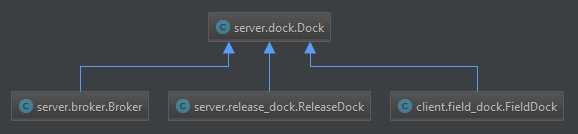
\includegraphics[scale=0.7]{afbeelding/classDock.png}}
%\caption{Klassendiagram van Dock}
%\label{fig:classDock}
%\end{figure}
%
%\paragraph{Grafische User Interfaces}
%Het is ook mogelijk om de Grafische User Interface (GUI) op te starten door middel van de ``Enter'' toets.
%Vanuit de GUI is het mogelijk om de verschillende clients te controleren en is het mogelijk om nieuwe installers te creëren.
%De GUI werd gemaakt met de Python bibliotheek wxPython\footnote{\url{https://wxpython.org/}} en met de hulp van wxFormBuilder\footnote{\url{https://github.com/wxFormBuilder/wxFormBuilder}} werd basis code gegenereerd.
%De nodige methodes werden vervolgens overschreven in de module overview\_impl.
%Via deze methode wordt een gelijkaardig resultaat behaald voor het maken van de GUI voor de installer creatie.
%
%\paragraph{Berichten versturen}
%Bij het versturen van een bericht moet eerst een object aangemaakt worden van de Message klasse.
%Vervolgens wordt de inhoud toegevoegd aan het bericht en kan het verzonden worden naar de broker.
%In de broker wordt gecontroleerd welk type bericht het is om het dan vervolgens door te sturen naar alle doelen die in de gepaste list zitten.
%Voordat het bericht wordt doorgestuurd wordt het eerst ingepakt in een ander bericht met als type notificatie.
%Zo weet de ontvanger dat het bericht afkomstig is van de broker en is weet de ontvanger dat het data veld het doorgestuurde bericht bevat.
%Deze kan vervolgens uitgepakt worden.
%Afhankelijk van het type van het doorgestuurde bericht zal de correcte methode opgeroepen worden.
%
%\paragraph{Installer creatie}
%In de overzicht GUI is het mogelijk om een nieuwe installer te maken.
%Met behulp van de aparte GUI, die geïmplementeerd wordt door de module release\_creator\_impl, is het mogelijk om een installer te definiëren.
%Tijdens het samenstellen van de installer kunnen verscheidene nieuwe pakketten aangemaakt worden door de bovenste velden meermaals in te vullen.
%Hierbij is het belangrijk om te weten dat een folder moet geselecteerd worden als bestandslocatie.
%Alle bestanden aanwezig in de geselecteerde folder worden tijdens de creatie verplaatst naar de correcte locatie.
%Bij het invullen van de gegevens van de installer moet ook een folder geselecteerd worden waarin de installer moet terecht komen.
%
%Bij het indienen van de gegevens van de installer zelf worden de nodige handelingen uitgevoerd om een correcte installer te produceren.
%Eerst worden de pakketten en installer toegevoegd aan de databank.
%Vervolgens wordt de nodige folder structuur opgebouwd zoals aangegeven werd in Figuur~\vref{fig:installerStructuur}.
%In de config folder wordt een leeg Dockerfile en een metadata bestand met daarin de volledige beschrijving van de installer.
%
%Van zodra in de overview GUI het release signaal gegeven wordt, schiet het tweede deel van het release proces in werking.
%Een install agent wordt aangemaakt en wordt toegevoegd aan de lijst van agenten horende bij de installer.
%De folder structuur uit het eerste deel wordt gezipt zodanig dat minder data verzonden moet worden.
%Als laatste deel van wordt een ``release'' bericht aangemaakt en verzonden naar de broker.
%Deze schiet vervolgens in gang en stuurt het bericht door naar de nodige field docks.
%
%\paragraph{Client monitoring}
%In de applicatie is het mogelijk om in een beperkte manier de clients te controleren.
%De overview GUI bevat een tabel met de verschillende clients die aanwezig zijn in de databank.
%Met hulp van de mysql.connector module van Python lukt het om de databank te ondervragen.
%Alle gegevens over de torens wordt opgevraagd en vervolgens worden er Tower objecten van gemaakt.
%Hierna wordt gecontroleerd of op de toren een installer aanwezig is.
%Mocht dit zo zijn, worden de gegevens over deze installer uit de databank gehaald.
%Op deze manier kan nagekeken worden welke installer aanwezig is en kan dit worden weergegeven in de GUI.
%
%\section{Client-side}
%\paragraph{Initialisatie}
%Aan de client-side wordt een gelijkaardige werkwijze gebruikt als bij de server-side.
%De module deployment\_client zal een field dock object aanmaken en de nodige services aanpassen.
%Tijdens het eerste gebruik van de code wordt een controle uitgevoerd waarmee gecontroleerd wordt of de description\_file aanwezig is.
%Dit bestand bevat de volledige beschrijving van de testtoren met alle verschillende hardware componenten.
%Vervolgens gaat het field dock zich subscriben voor de nodige berichten bij de broker.
%Als beide stappen zijn afgelopen, wordt de Grafische User Interface opgestart en is het systeem klaar om gebruikt te worden.
%
%\paragraph{Eerste gebruik}
%Bij het eerste gebruik van de applicatie is de description\_file nog niet aanwezig.
%Er is dan nog geen beschrijving van de gebruiker aanwezig aan zowel de client- als server-side.
%Om dit aan te pakken, wordt een GUI opgestart waarmee het mogelijk is om het volledige systeem te beschrijven.
%Na het invullen van de nodige informatie en het indienen van alle gegevens, wordt de description\_file aangemaakt.
%Een ``new'' bericht wordt gefabriceerd met in het data veld de volledige beschrijving van het systeem.
%Dit bericht wordt verzonden naar de broker en de broker stuurt het bericht door naar iedereen die gesubscribed is voor de ``new'' berichten.
%Het bericht komt toe bij het release dock.
%Het bericht wordt uitgepakt, omgevormd naar een Tower object en vervolgens toegevoegd aan de databank.
%
%\paragraph{Installatieproces}
%Van zodra een ``release'' bericht binnen komt bij het field dock schiet deze in gang om het installatieproces op poten te zetten.
%
%Dill\footnote{\url{https://pypi.python.org/pypi/dill}} wordt gebruikt om de agent objecten te serialiseren voor ze verzonden worden naar het field dock.
%
%De eerste actie die de install agent gaat ondernemen is het uitpakken van het zip bestand.
%Met de Dockerfile uit de installer en de docker-py\footnote{\url{https://docker-py.readthedocs.io/en/stable/}} module wordt een Docker image aangemaakt die de basis zal vormen voor de container.
%Voor de presentatie werd een image aangemaakt voor een Linux container waarin Python en wxPython op voorhand waren geïnstalleerd.
%Vervolgens wordt een container gecreëerd met als naam ``fieldcontainer''.
%Dit is de hoofdcontainer die altijd de laatst werkende versie van het framework zal bevatten.
%Tijdens de creatie werden de nodige parameters doorgegeven om Grafische User Interfaces van de container op te kunnen starten.
%Om dit mogelijk te maken, is het nodig om aan X11 forwarding te doen.
%Belangrijk hierbij is dat op de host computer een X11 server moet draaien voordat dit kan plaats vinden.
%Voor de demonstratie werd Cygwin\footnote{\url{https://www.cygwin.com/}} gebruikt om de X11 server op te starten en de correcte omgeving te generen\footnote{De tutorial \url{https://manomarks.net/2015/12/03/docker-gui-windows.html} werd hiervoor gevolgd}.
%Hierna wordt het metadata bestand gelezen en gebruikt om de installatievolgorde van de pakketten te achterhalen.
%Elk pakket wordt in de container gekopieerd en het installatie script wordt uitgevoerd.
%Vervolgens gaat, met hulp van het test script, nagegaan worden of het installatieproces correct verlopen is.
%De output van het script wordt gecontroleerd.
%Als de uitgangsstatus begint met 0 wordt de test gezien als geslaagd.
%Van zodra dit niet het geval is, wordt de container gemerkt als slecht en zal deze op het einde van het installatieproces in quarantaine geplaatst worden.
%De container wordt niet verwijdert. 
%Er werd voor deze strategie gekozen aangezien het mogelijk dat het test script slecht geschreven is.
%Het framework is dan correct geïnstalleerd maar wordt door de test toch gezien als foutief.
%Door de container in quarantaine te plaatsen blijft het mogelijk om achteraf test uit te voeren.
%Vervolgens wordt een rapport aangemaakt met daarin het resultaat van de test, de begin- en eindtijd.
%Het rapport wordt toegevoegd aan een bericht en wordt verzonden naar de broker die het doorstuurt.
%
%\paragraph{Framework opstarten}
%Na het opstarten van alle services verschijnt de Grafische User Interface van de client.
%Van hieruit is het mogelijk om het pakket dat gemarkeerd staat als framework te openen.
%De ``fieldcontainer'' wordt opgestart en het start script wordt uitgevoerd waardoor het framework zal opstarten.